\documentclass{resume}
\usepackage{geometry}

% Adjust the top margin to create more space for the image
\geometry{top=0.25in}

\begin{document}

\fontfamily{ppl}\selectfont

% Add negative \vspace to move the content up
\vspace*{-0.6cm}

\noindent
\begin{tabularx}{\linewidth}{@{}m{0.8\textwidth} m{0.175\textwidth}@{}}
{
    \Large{Chetan Sarigala} \newline
    \small{
        \clink{
            \href{mailto:cs20b1019@iiitr.ac.in}{CS20B1019@iiitr.ac.in} \textbf{·} 
            {\fontdimen2\font=0.75ex +91 9391719199} 
        } \newline
        Hyderabad, India
    }
} & 
{
    \hfill
    % Increase the size of the image
    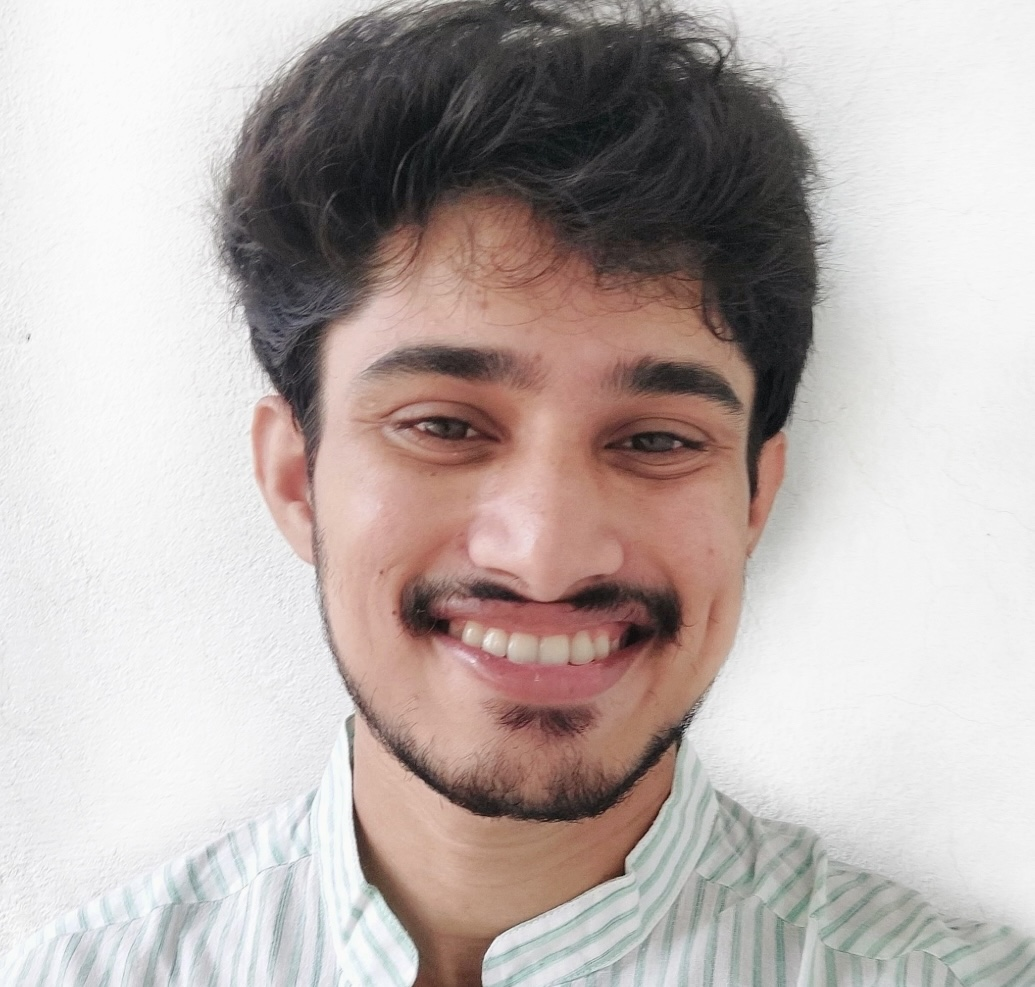
\includegraphics[width=3.2cm]{images/gr.png}
}
\end{tabularx}
\begin{center}
\begin{tabularx}{\linewidth}{@{}*{2}{X}@{}}
% left side %
{
    \csection{EXPERIENCE}{\small
        \begin{itemize}
            % item 1 %
            \item \frcontent{SabZ}{Internship - Agriculture and E-commerce, Hyderabad}{Joined a startup with 7 employees, focusing on data collection, analysis, and interpretation for decision-making. Notable skill gained: K-Means}{Dec 2021 - Jan 2022}
            % item 2 %
            \item \frcontent{Teaching Assistant}{Machine Learning, IIIT Raichur}{Assisted in a Machine Learning course, evaluated tests, and helped students with key concepts.}{Aug 2023 - Dec 2023}
            % item 3 %
            \item \frcontent{E-Cell Sponsor Head}{IIIT Raichur}{Managed sponsorships, negotiated MoUs, and handled legal considerations with companies and entrepreneurs.}{Aug 2023 - Dec 2023}
        \end{itemize}
    }
    \csection{EDUCATION}{\small
        \begin{itemize}
            % item 1 %
            \item \frcontent{B.Tech in Computer Science, CGPA: 6.45/10}{IIIT Raichur}{}{2020-2024}
            \item \frcontent{Intermediate, CGPA: 9.0/10}{Sri Chaitanya}{}{2018-2020}
        \end{itemize}
    }
    \csection{AWARDS \& RECOGNITION}{\small
        \begin{itemize}
            % item 1 %
            \item \frcontent{2nd Rank, Torque Auto-CAD Logo Design}{IIT Hyderabad}{}{2021}
            % item 2 %
            \item \frcontent{1st Rank, Design Competition using Coding}{IIIT Raichur}{}{2022}
            % item 3 %
            \item \frcontent{Reached Round 1B in CodeChef Global Programming Competition}{}{}{2021}
        \end{itemize}
    }
} 
% end left side %
& 
% right side %
{
    \csection{SKILLS}{\small
        \begin{itemize}
            \item \textbf{Technologies} \newline
            {\footnotesize Python, Machine Learning, Deep Learning, NLP, Large Language Models}{}{}
        \end{itemize}
    }
    \csection{PROJECTS}{\small
        \begin{itemize}
            \item \frcontent{Optimizing Intent Classification Using Joint BERT: A Comparative Study with GPT and LSTM\clink{\href{https://github.com/SarigalaChetan/Analysis-of-Similarity-Metrics-in-Text-Classification..git}{[github.com]}}}{Compared GPT, LSTM, and BERT in intent classification, integrating the best model in a joint model for improved results.}{}{Pandas, NumPy, TensorFlow, Scikit-learn, BERT, GPT, LSTM}
            \item \frcontent{SQL Query Generation and Correction \clink{\href{https://github.com/SarigalaChetan/SQL-Query-Generation-and-Correction.git}{[github.com]}}}{Proposed a new model combining T5 and Chatdb for query generation and correction, achieving higher accuracy than T5 and Chatdb}{}{Pandas, T5, chatdb, SQL}
            \item \frcontent{Analysis of Similarity Measurement Techniques on Text Documents \clink{\href{https://github.com/SarigalaChetan/Analysis-of-Similarity-Metrics-in-Text-Classification..git}{[github.com]}}}{Explored and compared various text similarity metrics like Cosine, Jaccard, SimRank and Others }{}{Pandas, NumPy, Scikit-learn, Matplotlib, SimRank}
        \end{itemize}
    }
    \csection{OTHER HIGHLIGHTS}{\small
        \begin{itemize}
            \item {\footnotesize Served as the Sports Secretary of IIIT Raichur, managing the team's participation in the Inter-IIIT event at IIIT Allahabad, securing 4 medals, and handling all related logistics and paperwork. Developed leadership and communication skills.}
        \end{itemize}
    }
    \csection{HOBBIES \& INTERESTS}{\small
    \vspace{0.32cm}
    \begin{itemize}
        \item \textbf{Drawing}
        \item \textbf{Chess}
        \item \textbf{Reading Articles (MoneyControl)}
    \end{itemize}
    }
}
\end{tabularx}
\end{center}
\end{document}